\documentclass{beamer}
\usepackage[utf8]{inputenc}

\usepackage{utopia} %font utopia imported


% There are many different themes available for Beamer. A comprehensive
% list with examples is given here:
% http://deic.uab.es/~iblanes/beamer_gallery/index_by_theme.html
% You can uncomment the themes below if you would like to use a different
% one:
%\usetheme{AnnArbor}
%\usetheme{Antibes}
%\usetheme{Bergen}
%\usetheme{Berkeley}
%\usetheme{Berlin} %good
%\usetheme{Boadilla}
%\usetheme{boxes}
%\usetheme{CambridgeUS}
%\usetheme{Copenhagen} %good
%\usetheme{Darmstadt} %good
%\usetheme{default}
%\usetheme{Frankfurt}
%\usetheme{Goettingen}
%\usetheme{Hannover}
%\usetheme{Ilmenau} %good
\usetheme{JuanLesPins} %g00d
%\usetheme{Luebeck}
%\usetheme{Madrid}
%\usetheme{Malmoe}
%\usetheme{Marburg}
%\usetheme{Montpellier}
%\usetheme{PaloAlto}
%\usetheme{Pittsburgh}
%\usetheme{Rochester}
%\usetheme{Singapore}
%\usetheme{Szeged}
%\usetheme{Warsaw}
\usecolortheme{beaver}
\usepackage{xcolor}
\usepackage{multirow}
\usebackgroundtemplate{%
	
		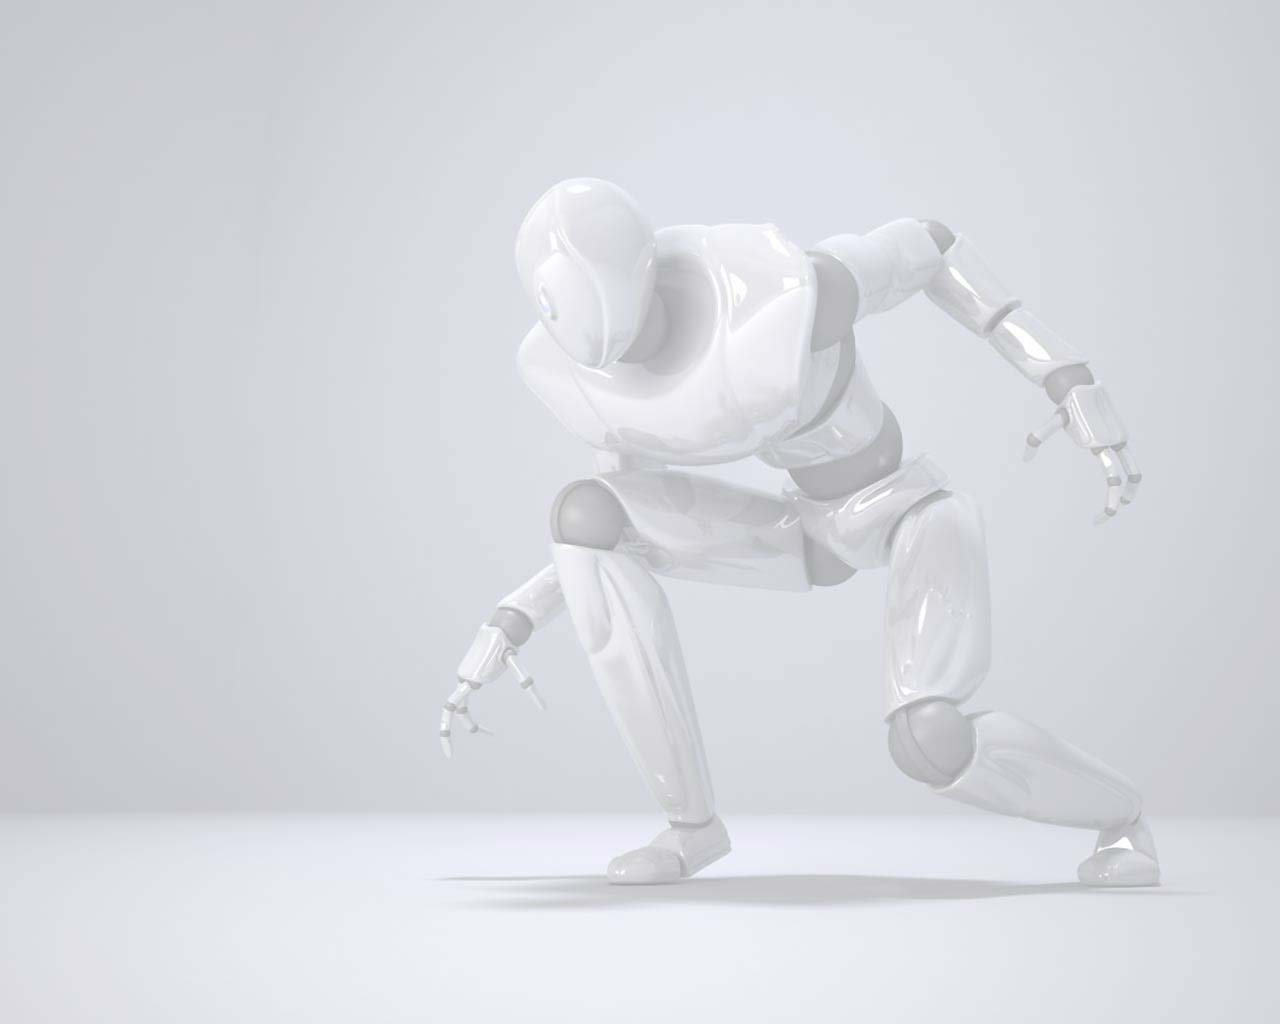
\includegraphics[height=\paperheight,width=\paperwidth]{Scorpio}
}
%------------------------------------------------------------
%This block of code defines the information to appear in the
%Title page
\title[Humanoid Robot] %optional
{Humanoid Robot}



\author[Vijay \and Jaipal] % (optional)
{Vijay Belurkar \and Jaipal Deval}

\institute[IITB] % (optional)
{
	%
	E-Yantra Summer Internship Program - 2014,\\
	IIT Bombay\\
	
}

\date[July 8 2014] % (optional)
{Mentors: Saurav Shandilya and Vishwanathan Iyer}

\logo{
\includegraphics[height=1.0cm]{iitlogo.jpg}}



%End of title page configuration block
%------------------------------------------------------------

\subject{Humanoid Robot}

% This is only inserted into the PDF information catalog. Can be left
% out. 

% If you have a file called "university-logo-filename.xxx", where xxx
% is a graphic format that can be processed by latex or pdflatex,
% resp., then you can add a logo as follows:

% \pgfdeclareimage[height=0.5cm]{university-logo}{university-logo-filename}
% \logo{\pgfuseimage{university-logo}}

% Delete this, if you do not want the table of contents to pop up at
% the beginning of each subsection:





% Let's get started
\begin{document}

\begin{frame}

  \titlepage
\end{frame}

\begin{frame}{Outline}
  \tableofcontents
  % You might wish to add the option [pausesections]
\end{frame}

% Section and subsections will appear in the presentation overview
% and table of contents.
\section{Objective of the work}
\begin{frame}{Objective of the work}
\begin{itemize}
	\item Humanoid Robot with 16 DOFs
	\item Basic concepts of Humanoid robot.
	\item Basic movements.
	\item Servo interface with micro-controller
	\item Power supply.\\
	
	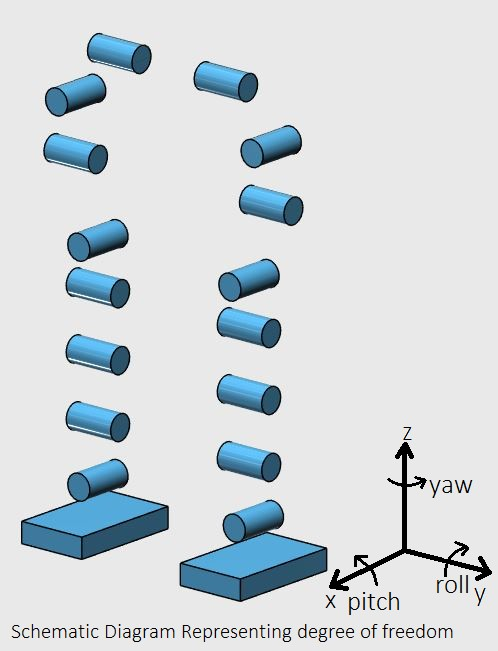
\includegraphics[width=2cm,height=3cm]{Schematic}
	\hspace{1cm}
	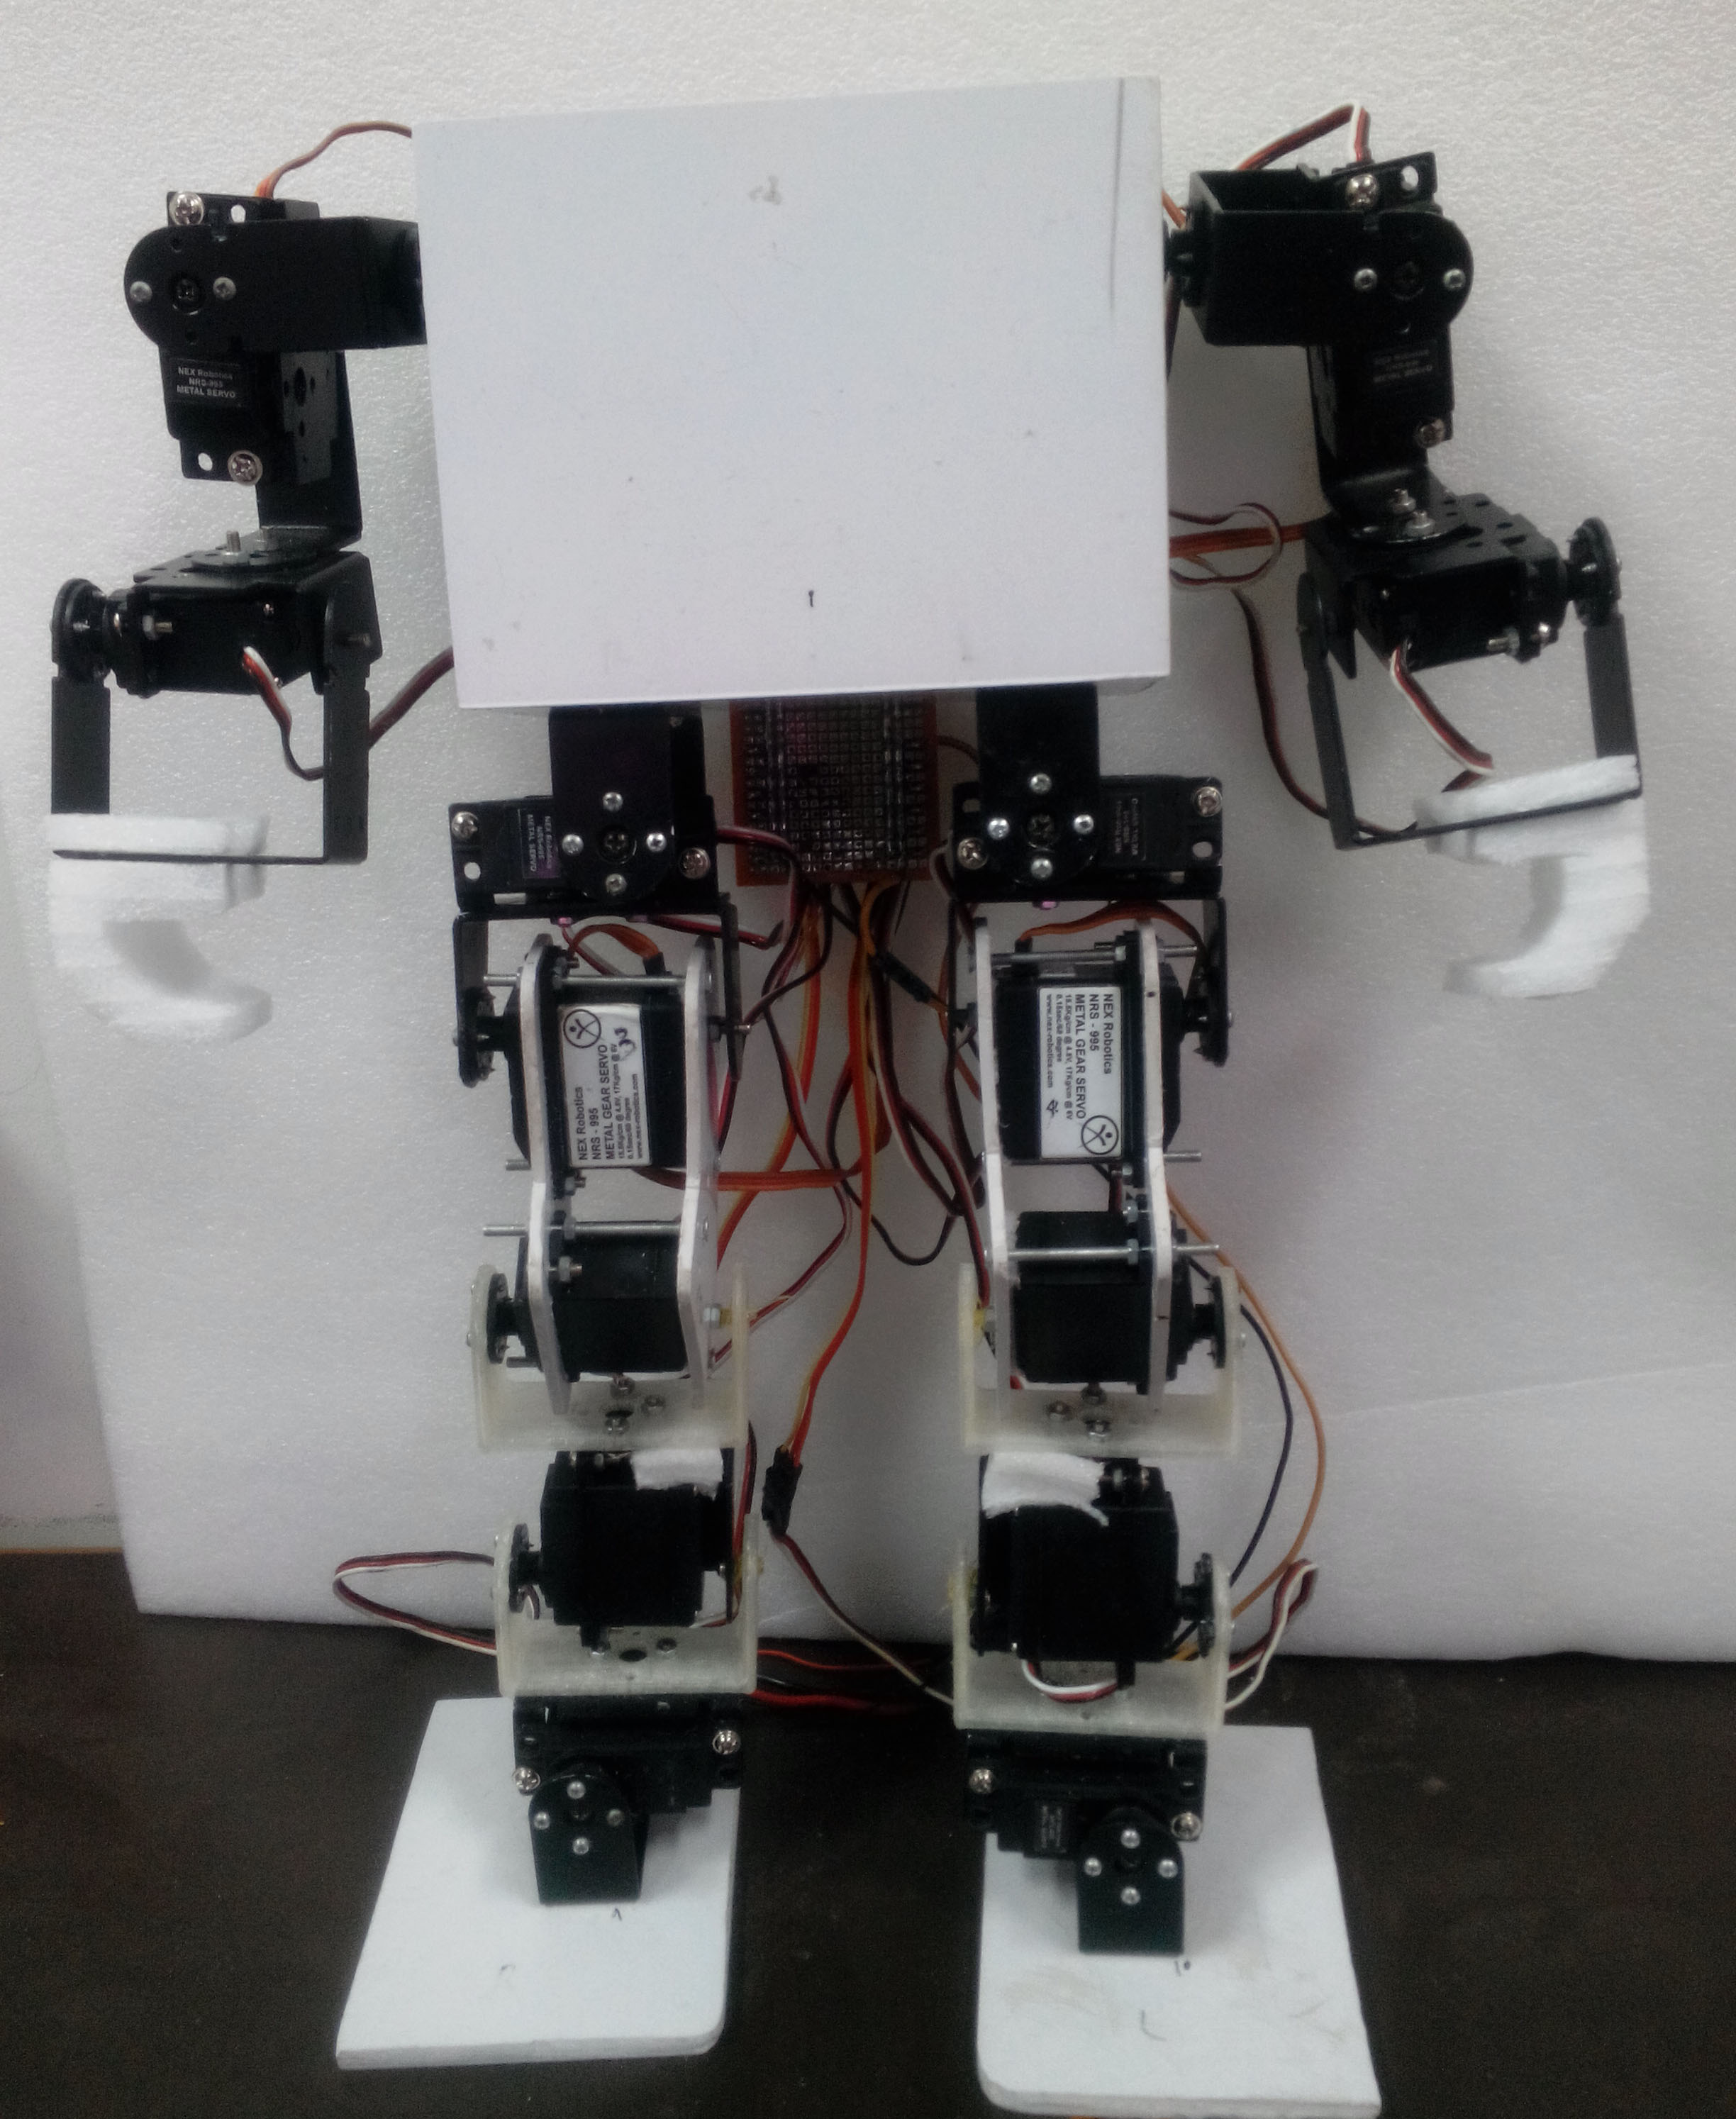
\includegraphics[width=2cm,height=3cm]{body_assembly}
\end{itemize}
\end{frame}

\section{Design}
\begin{frame}{Design}
\begin{columns}[c] % The "c" option specifies centered vertical alignment while the "t" option is used for top vertical alignment
	
	\column{.4\textwidth} % Left column and width
	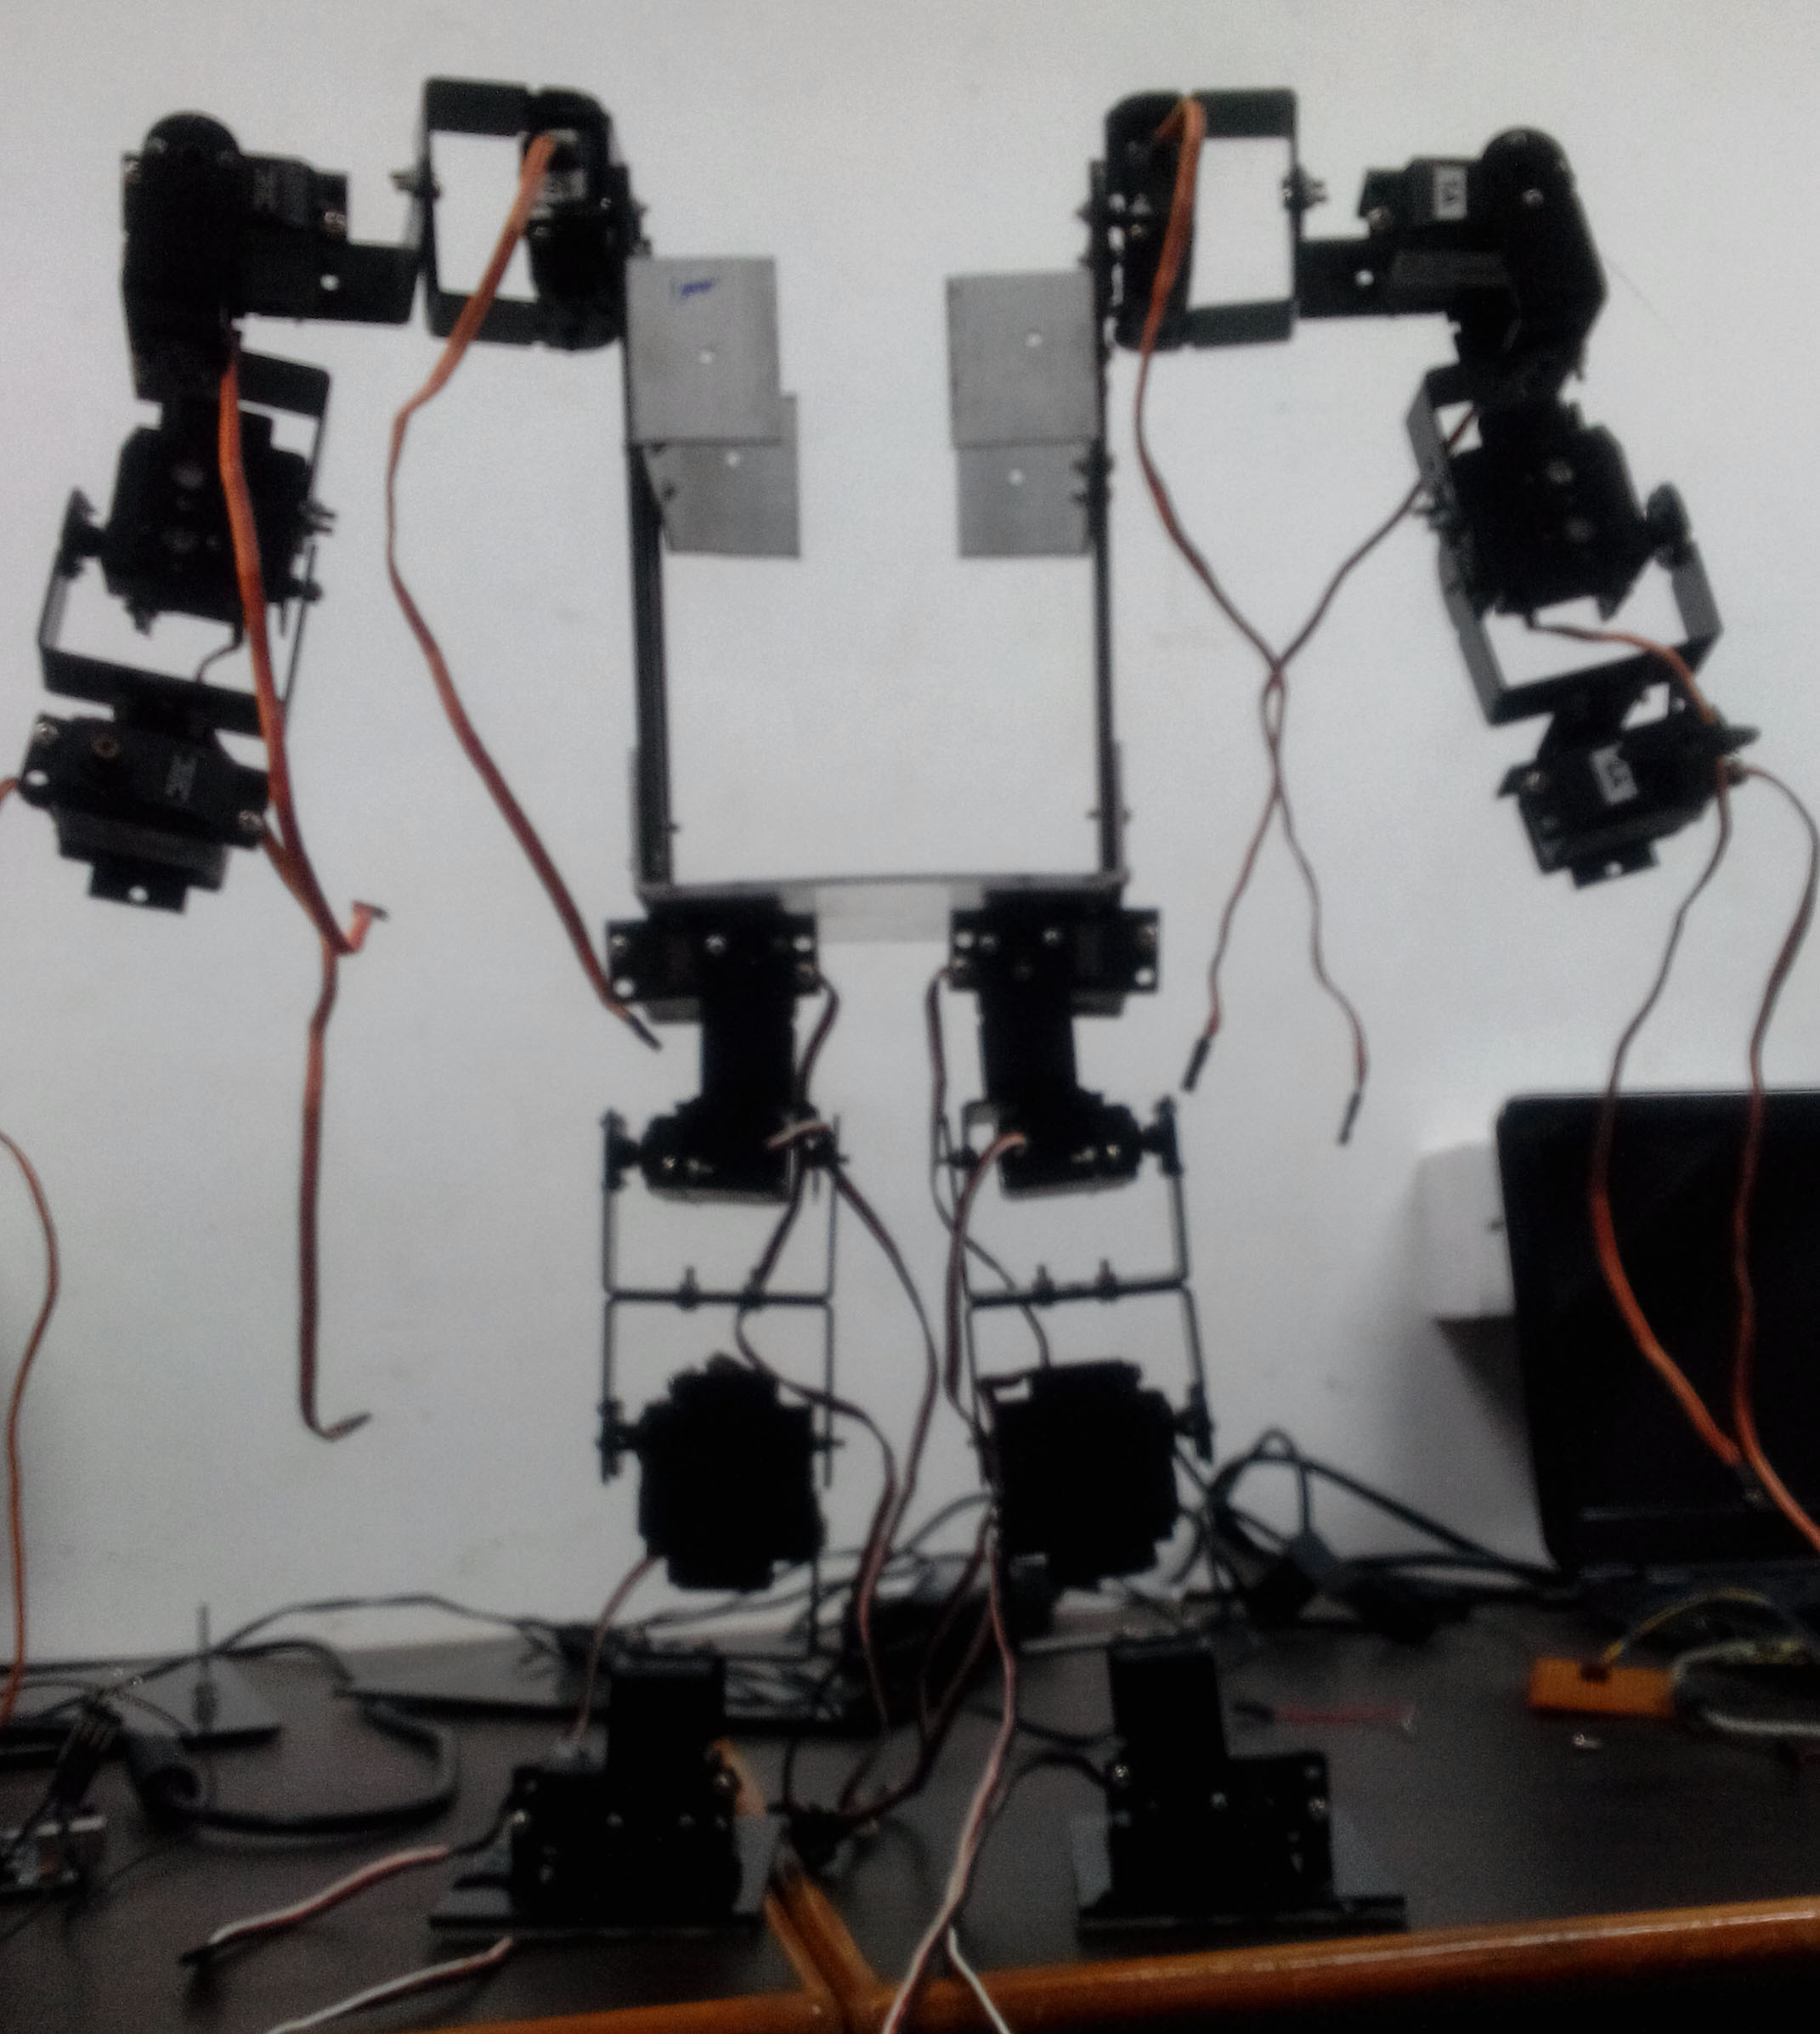
\includegraphics[width=3cm,height=4cm]{oned}
	\begin{enumerate}
		\item Size
		\item Bracket
		\item L clamp
	\end{enumerate}
	
	\column{.4\textwidth} % Right column and width
	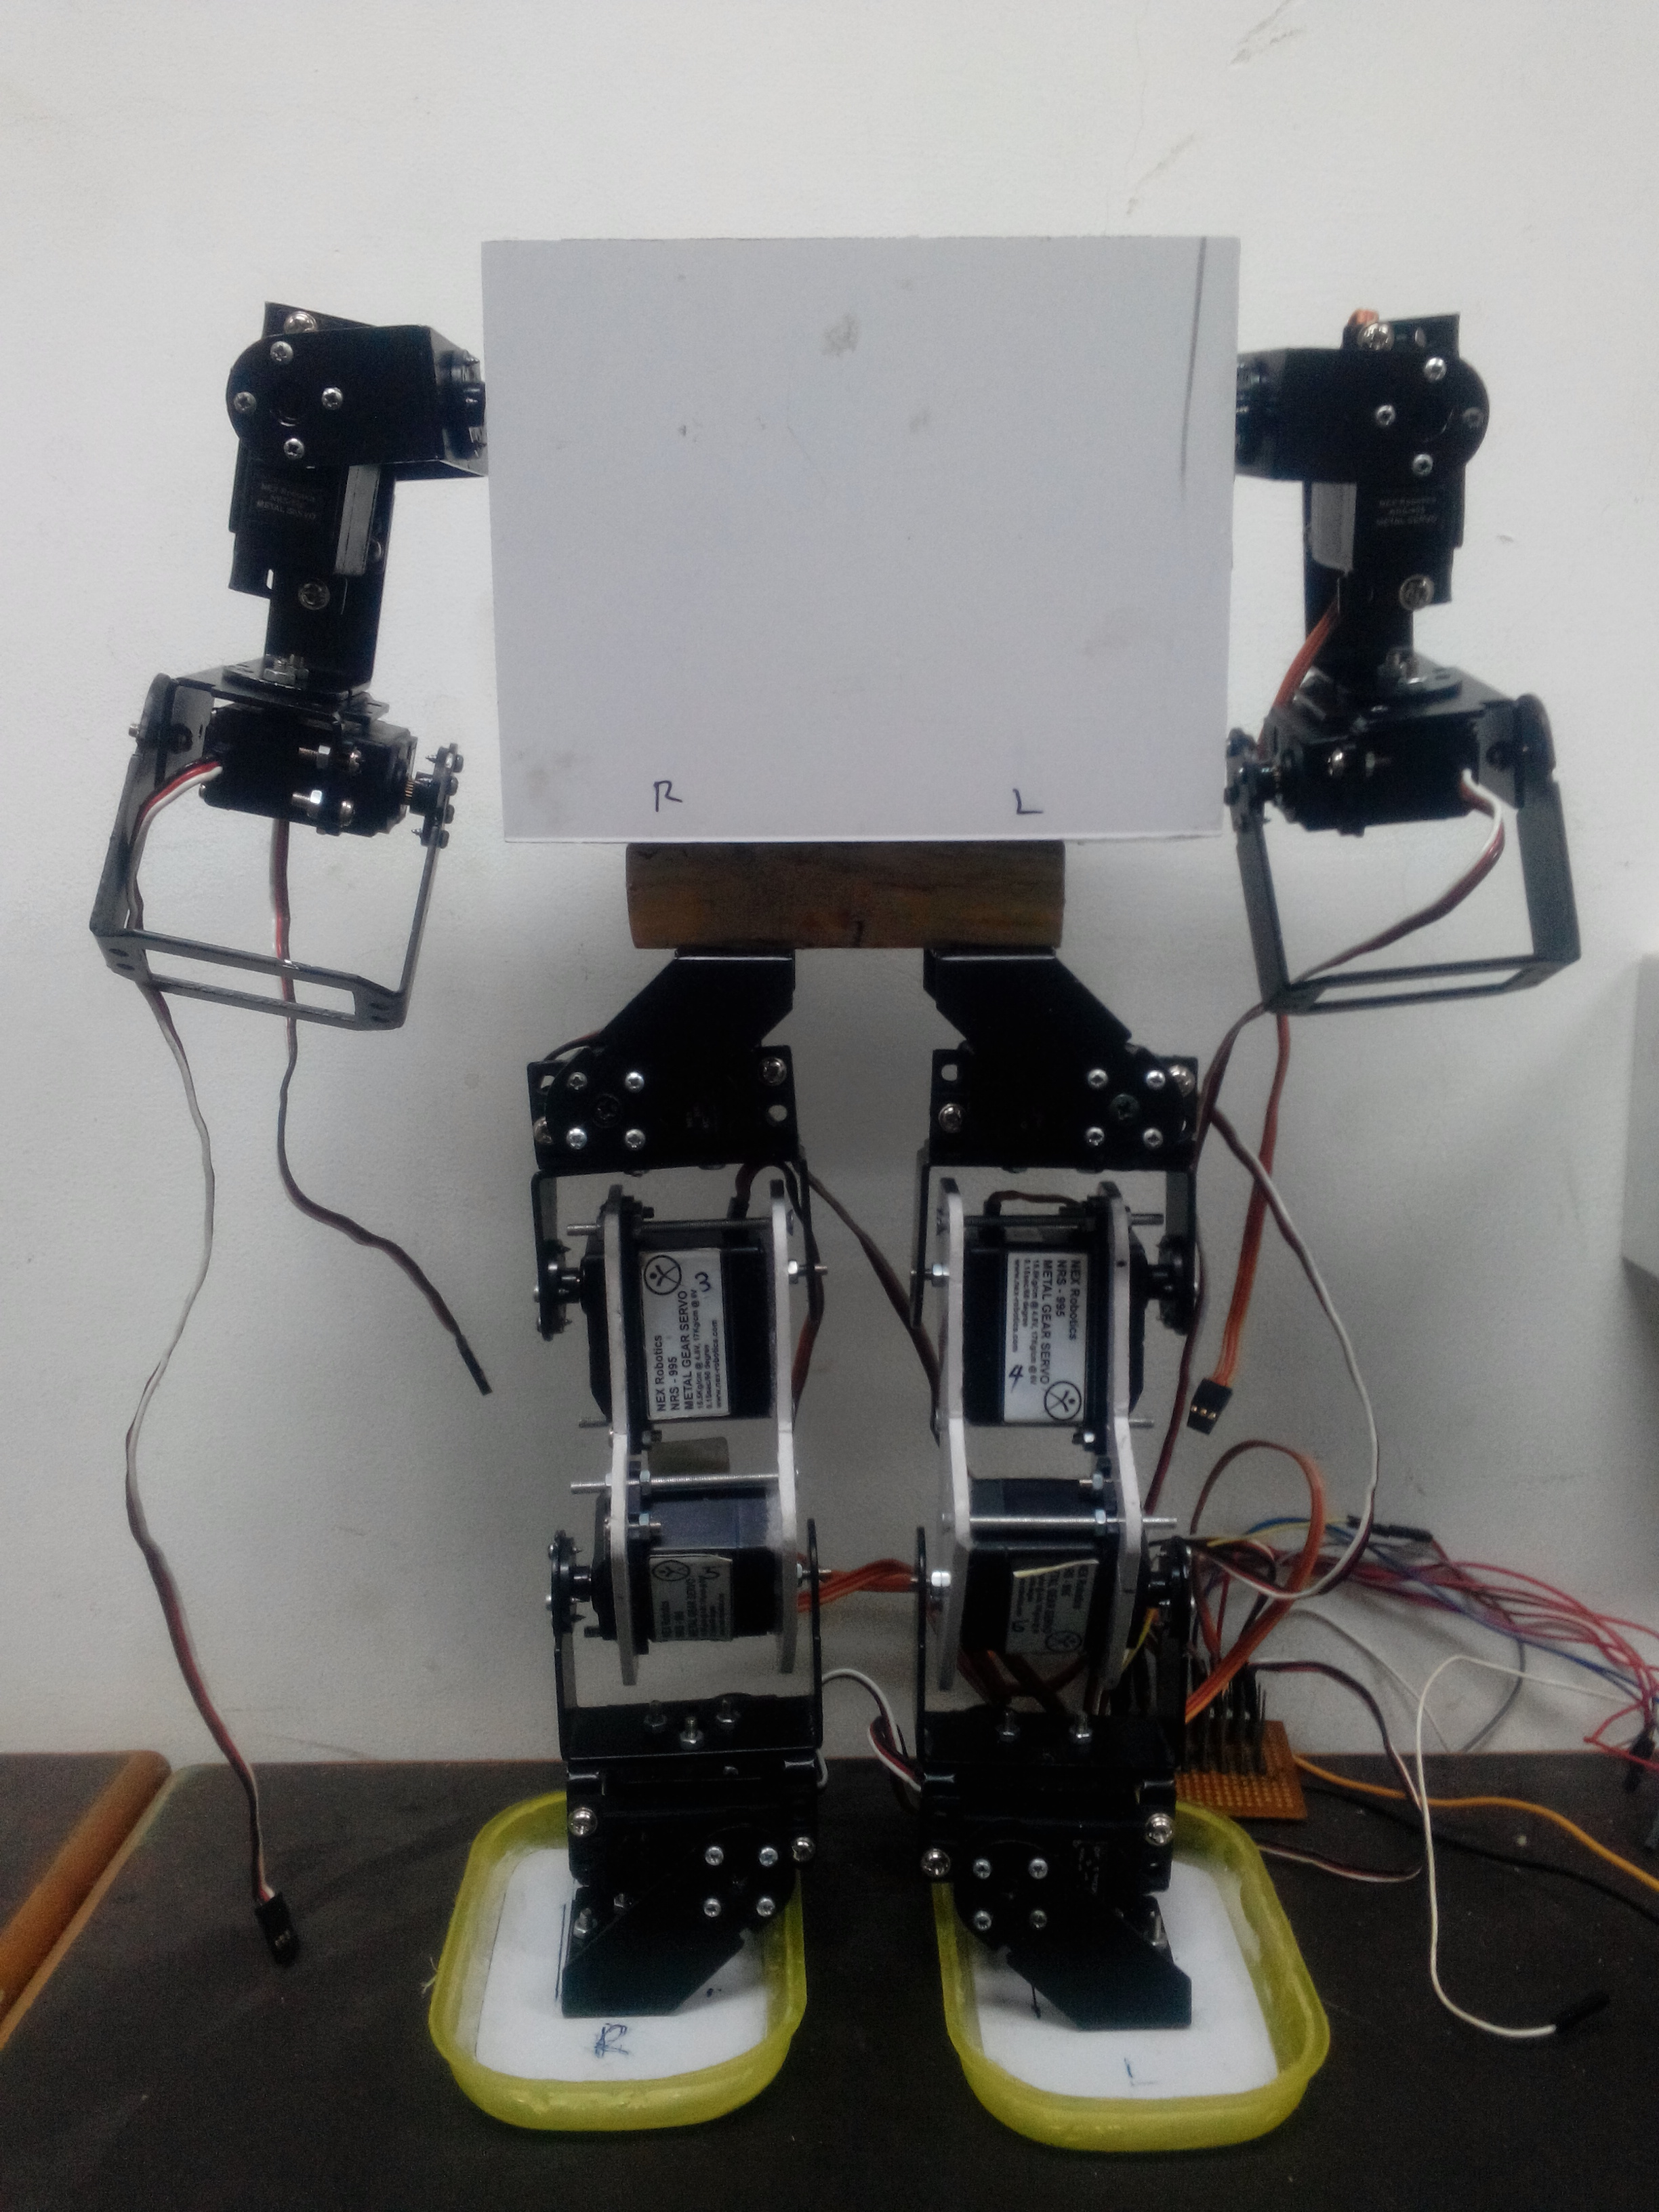
\includegraphics[width=3cm,height=4cm]{IMG_20140607_214454}
	\begin{enumerate}
		\item Walk
		\item Feet
		\item Angled clamp
	\end{enumerate}
	\column{.4\textwidth} % Right column and width
	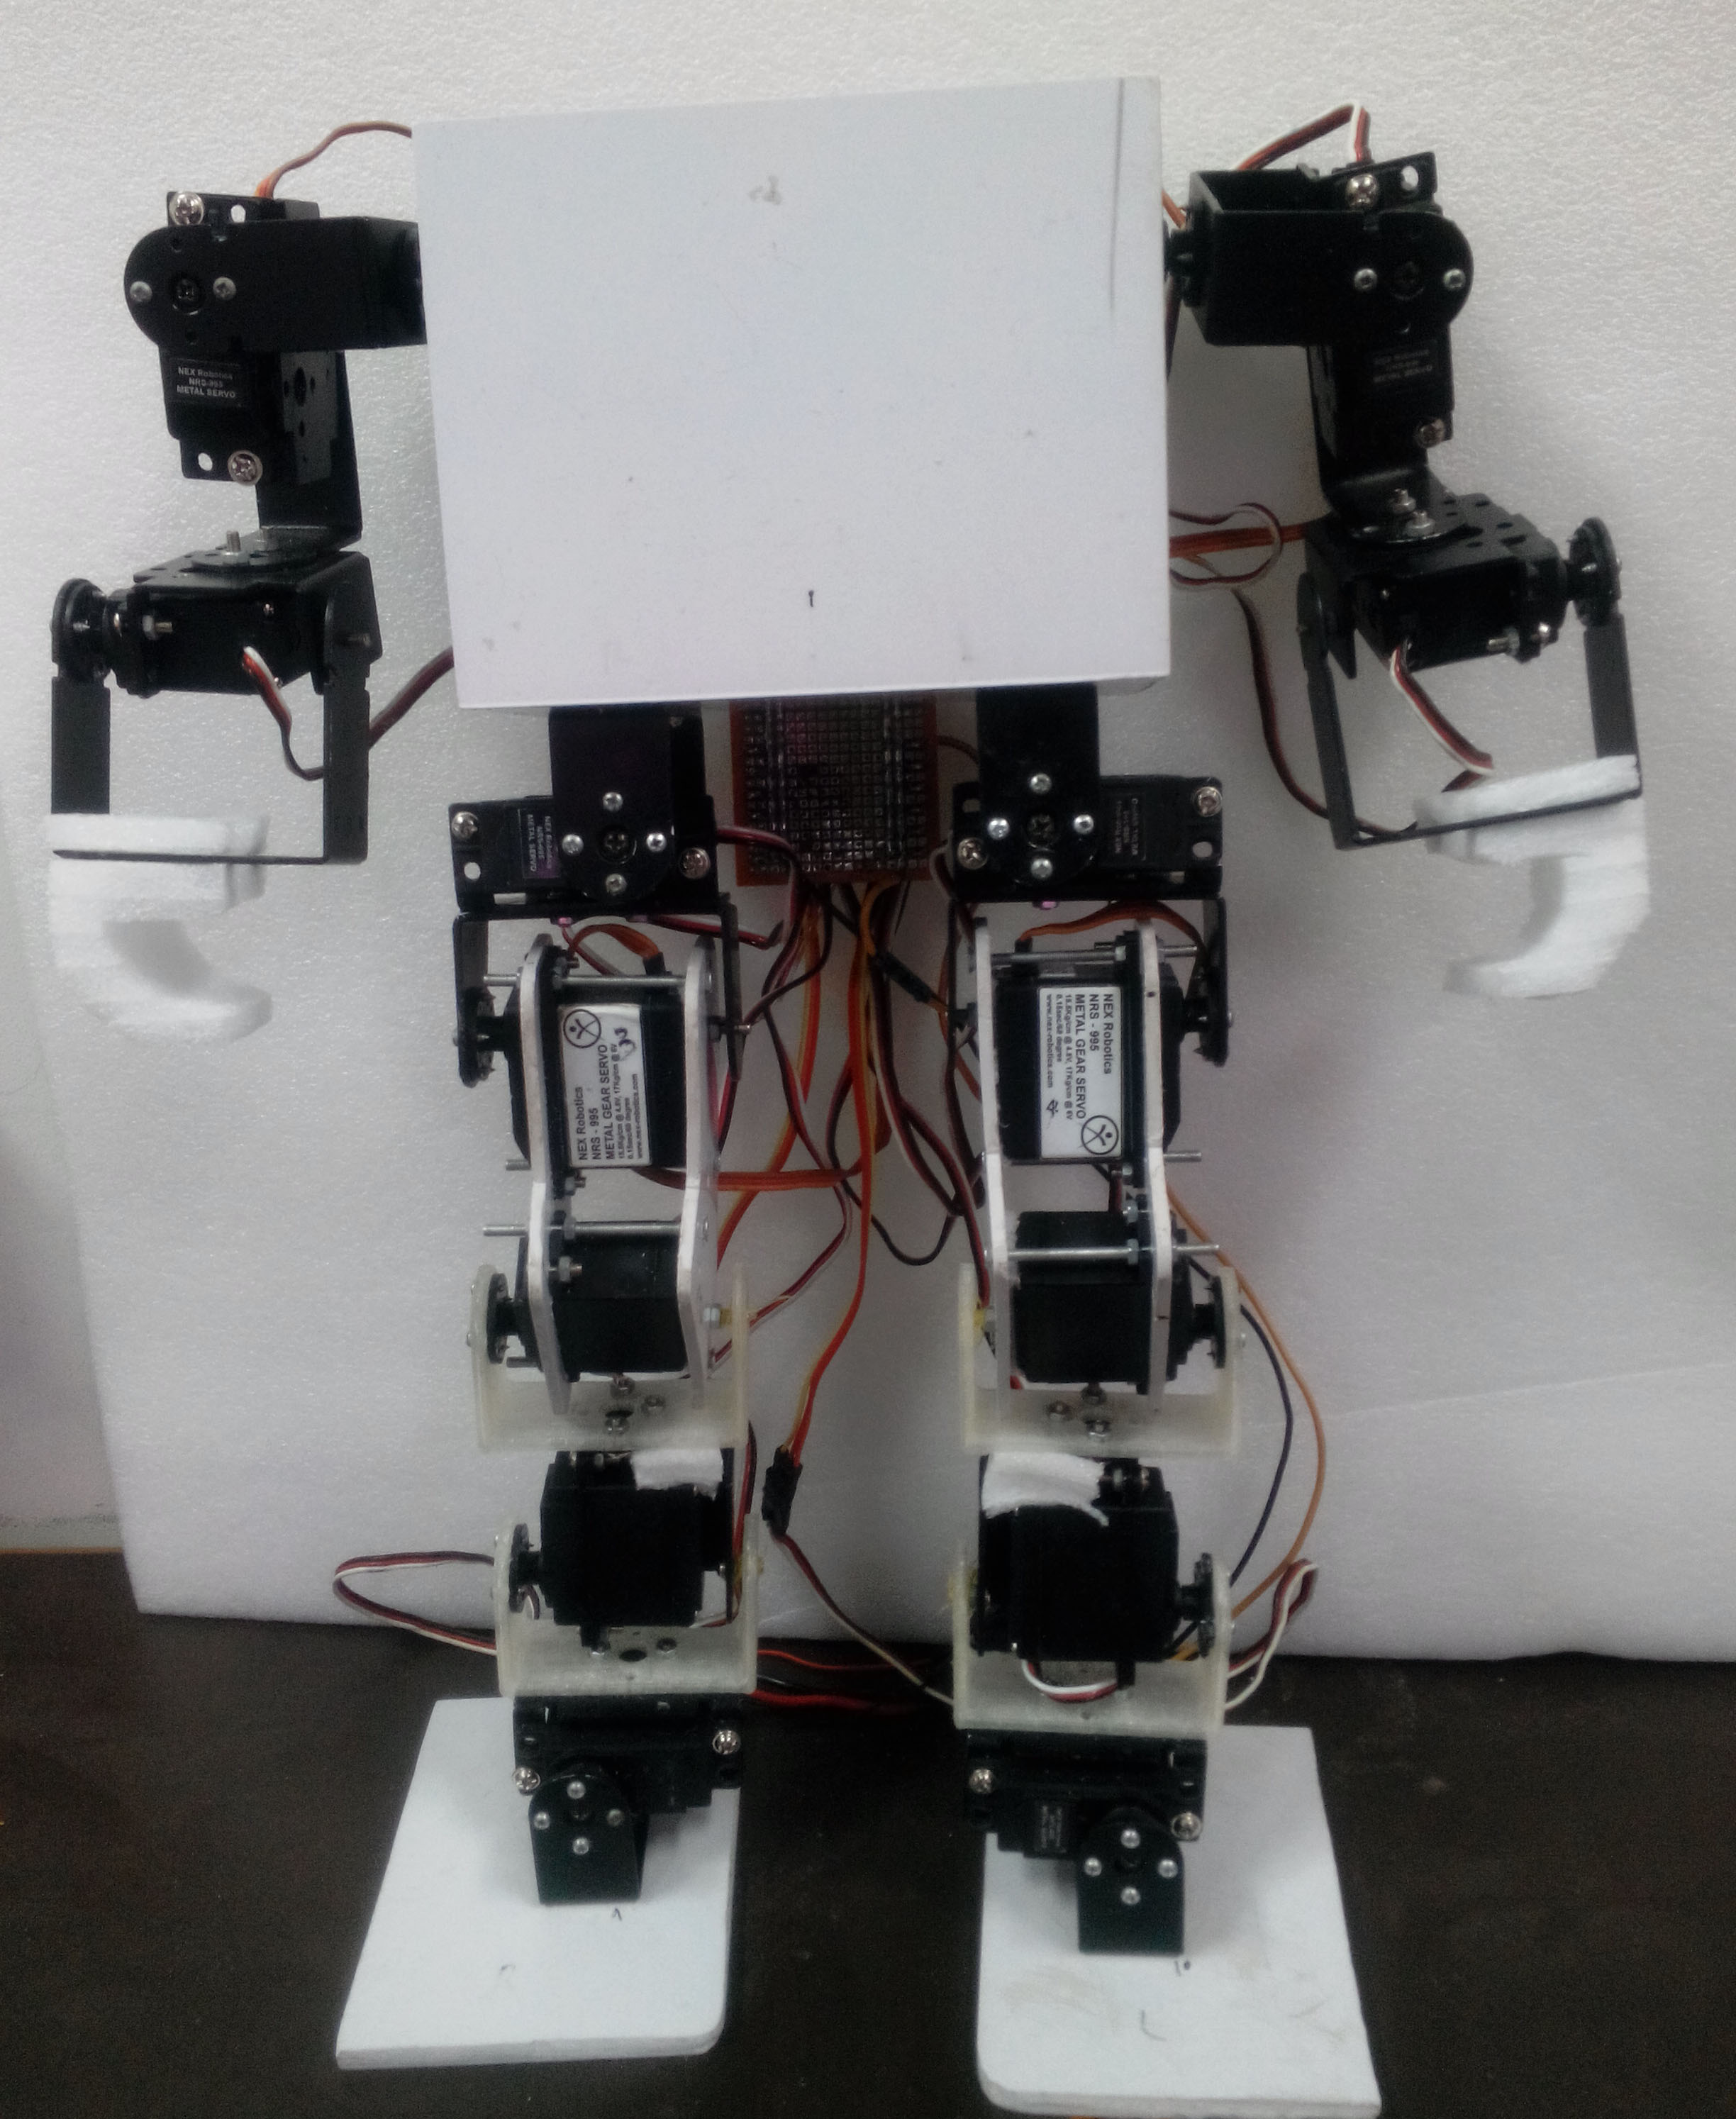
\includegraphics[width=3cm,height=4cm]{body_assembly}
	\begin{enumerate}
			\item Human walk
			\item Robust
			\item Flat feet
	\end{enumerate}
\end{columns}
\end{frame}

\section{Completion}
\begin{frame}
	\begin{itemize}
		\item[\checkmark]  Humanoid Robot with 16 DOFs was successfully constructed.
		\item[\checkmark] Servo motors were interfaced with ATMEGA 640
		\item[\checkmark] Basic concepts of Humanoid robot were studied.
		\item[\checkmark] Basic movements were programmed and tested successfully.
		\item[\checkmark] Suitable power supply was designed.\\
		
		
	\end{itemize}
\end{frame}

\section{Results}
\begin{frame}{Results}
	\begin{itemize}
		\item We were successfully able to achieve the following motions:
		\begin{itemize}
			\item[\checkmark] Basic Swing
			\item[\checkmark] Balancing on One leg (CG balance)
			\item[\checkmark] Kicking and hand movements
			\item[\checkmark] Sit-ups
			\item[\checkmark] Walking\\
		\end{itemize}
		\item Video Demonstrations
	\end{itemize}
\end{frame}


\section{Features \& bugs}
\begin{frame}{Features \& bugs}
	\begin{columns}[c]
		\column{.6\textwidth}
		\begin{itemize}
		\item \textbf{Features:}
		\begin{itemize}
			\item Robust
			\item Walking and other basic movements
			\item PWM using interrupts
		\end{itemize}
		
		\item \textbf{Bugs:}
		\begin{itemize}
			\item Metal gear Servo motors
			\item Battery cannot be accommodated
			\item Servo jittering during testing phase
			\item Servo plastic flaps
		\end{itemize}
	\end{itemize}
		\column{0.3\textwidth}
		
		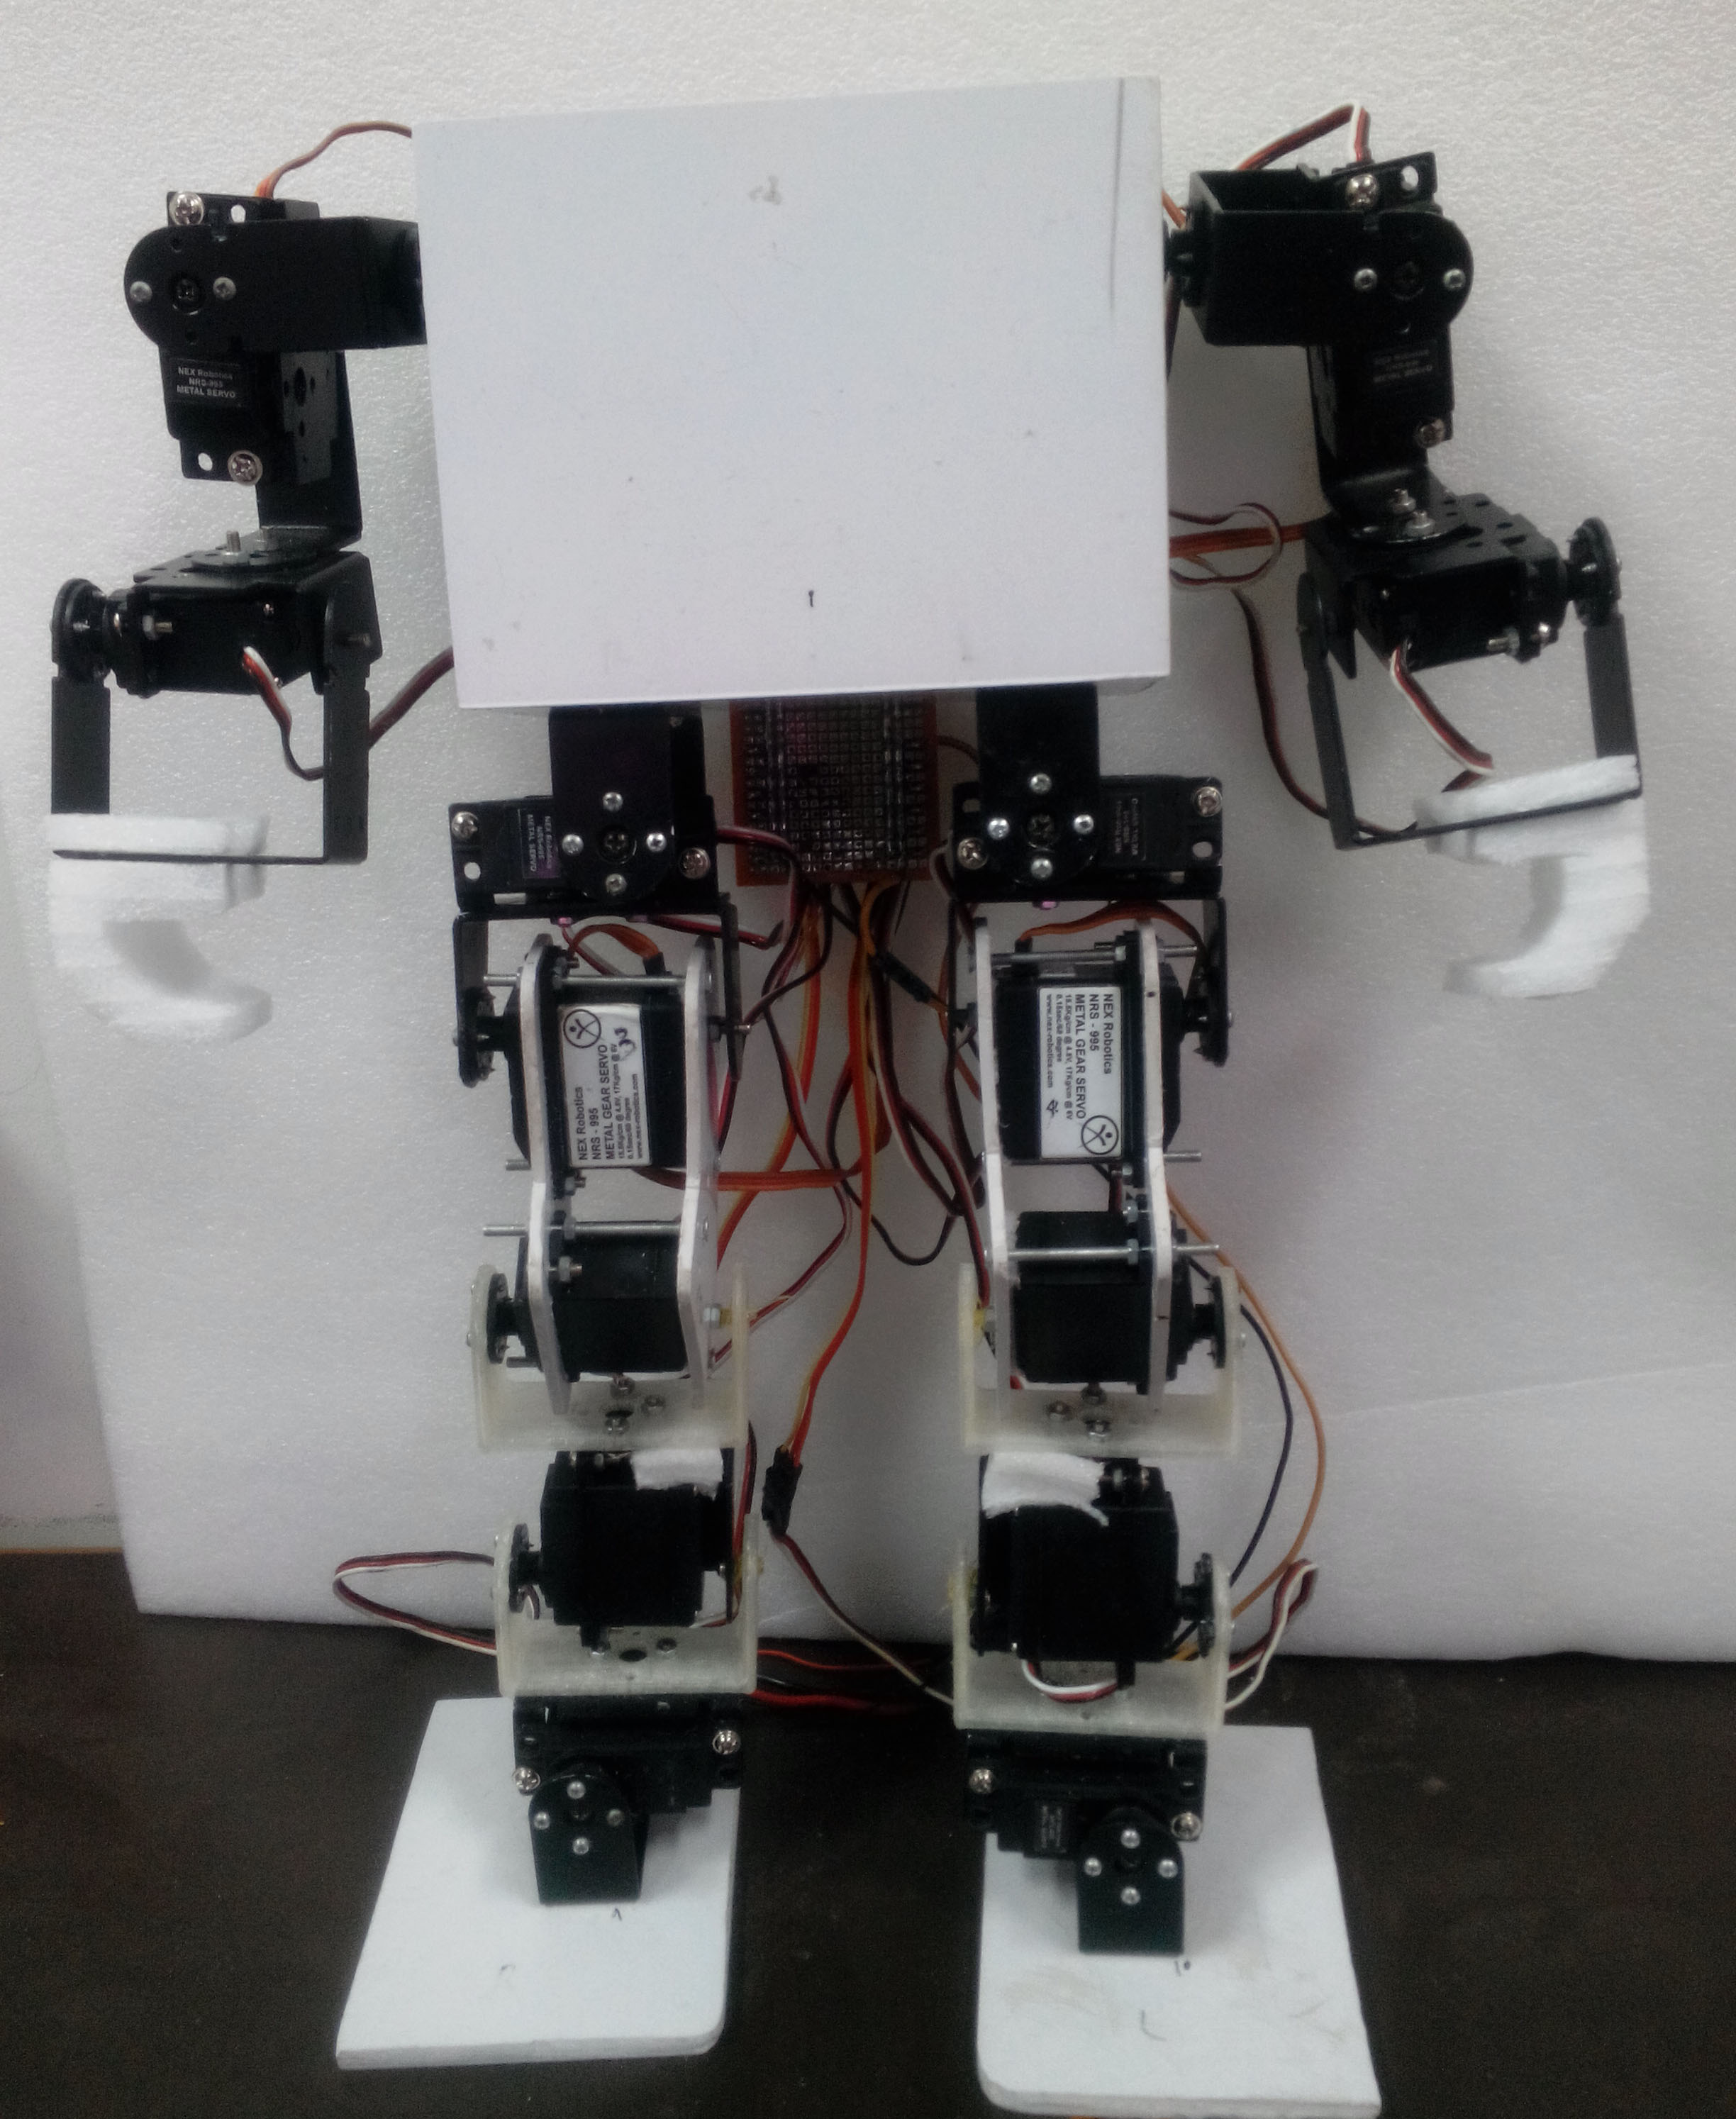
\includegraphics[width=3cm,height=4cm]{body_assembly}\\
		
	\column{0.3\textwidth}
	
	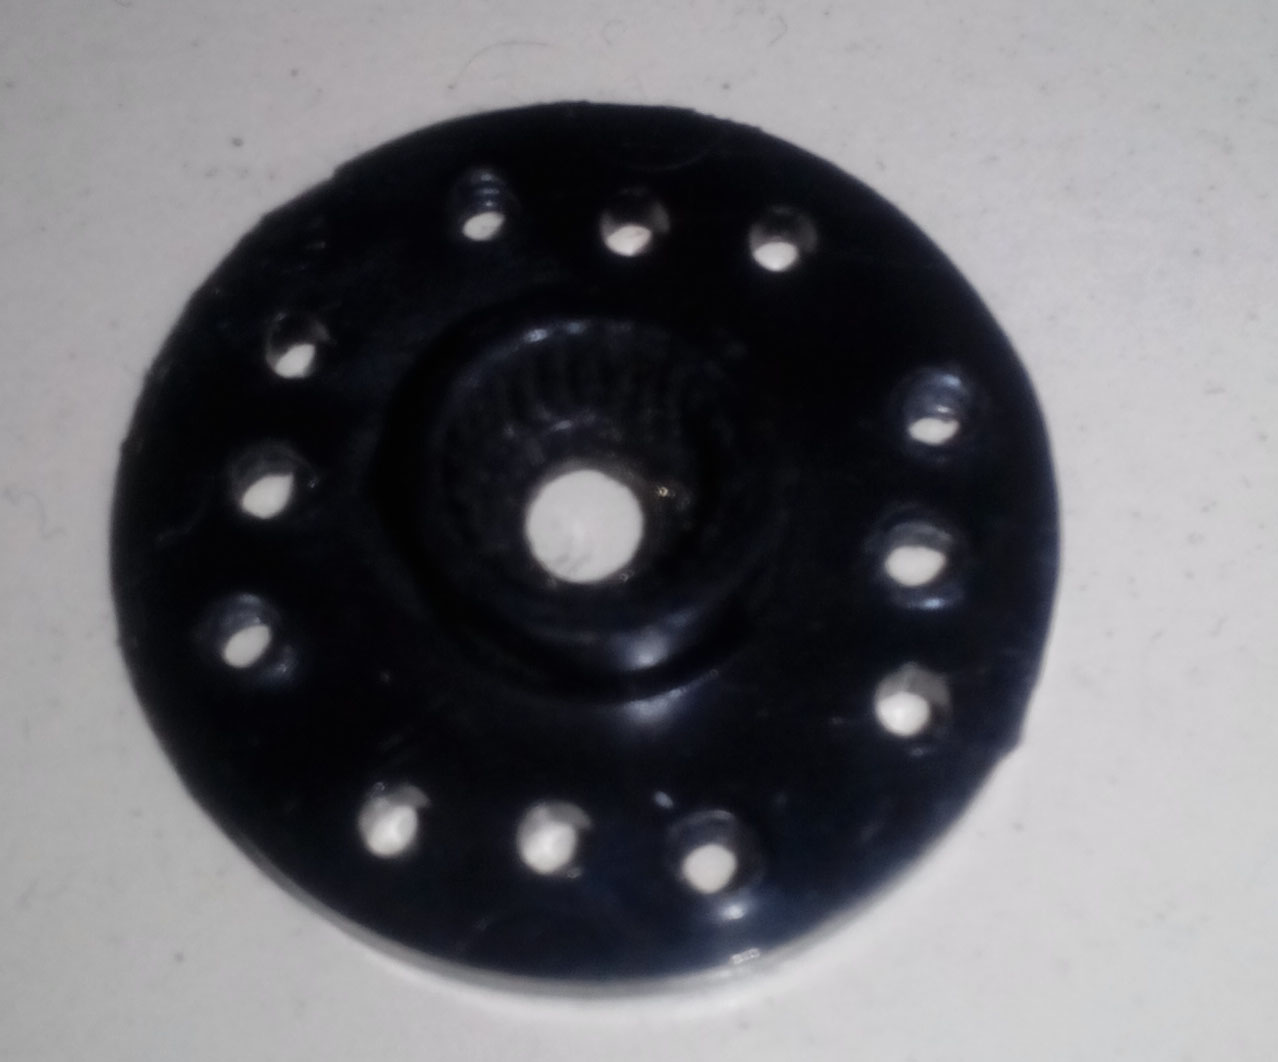
\includegraphics[width=3cm,height=3cm]{flap}\\
	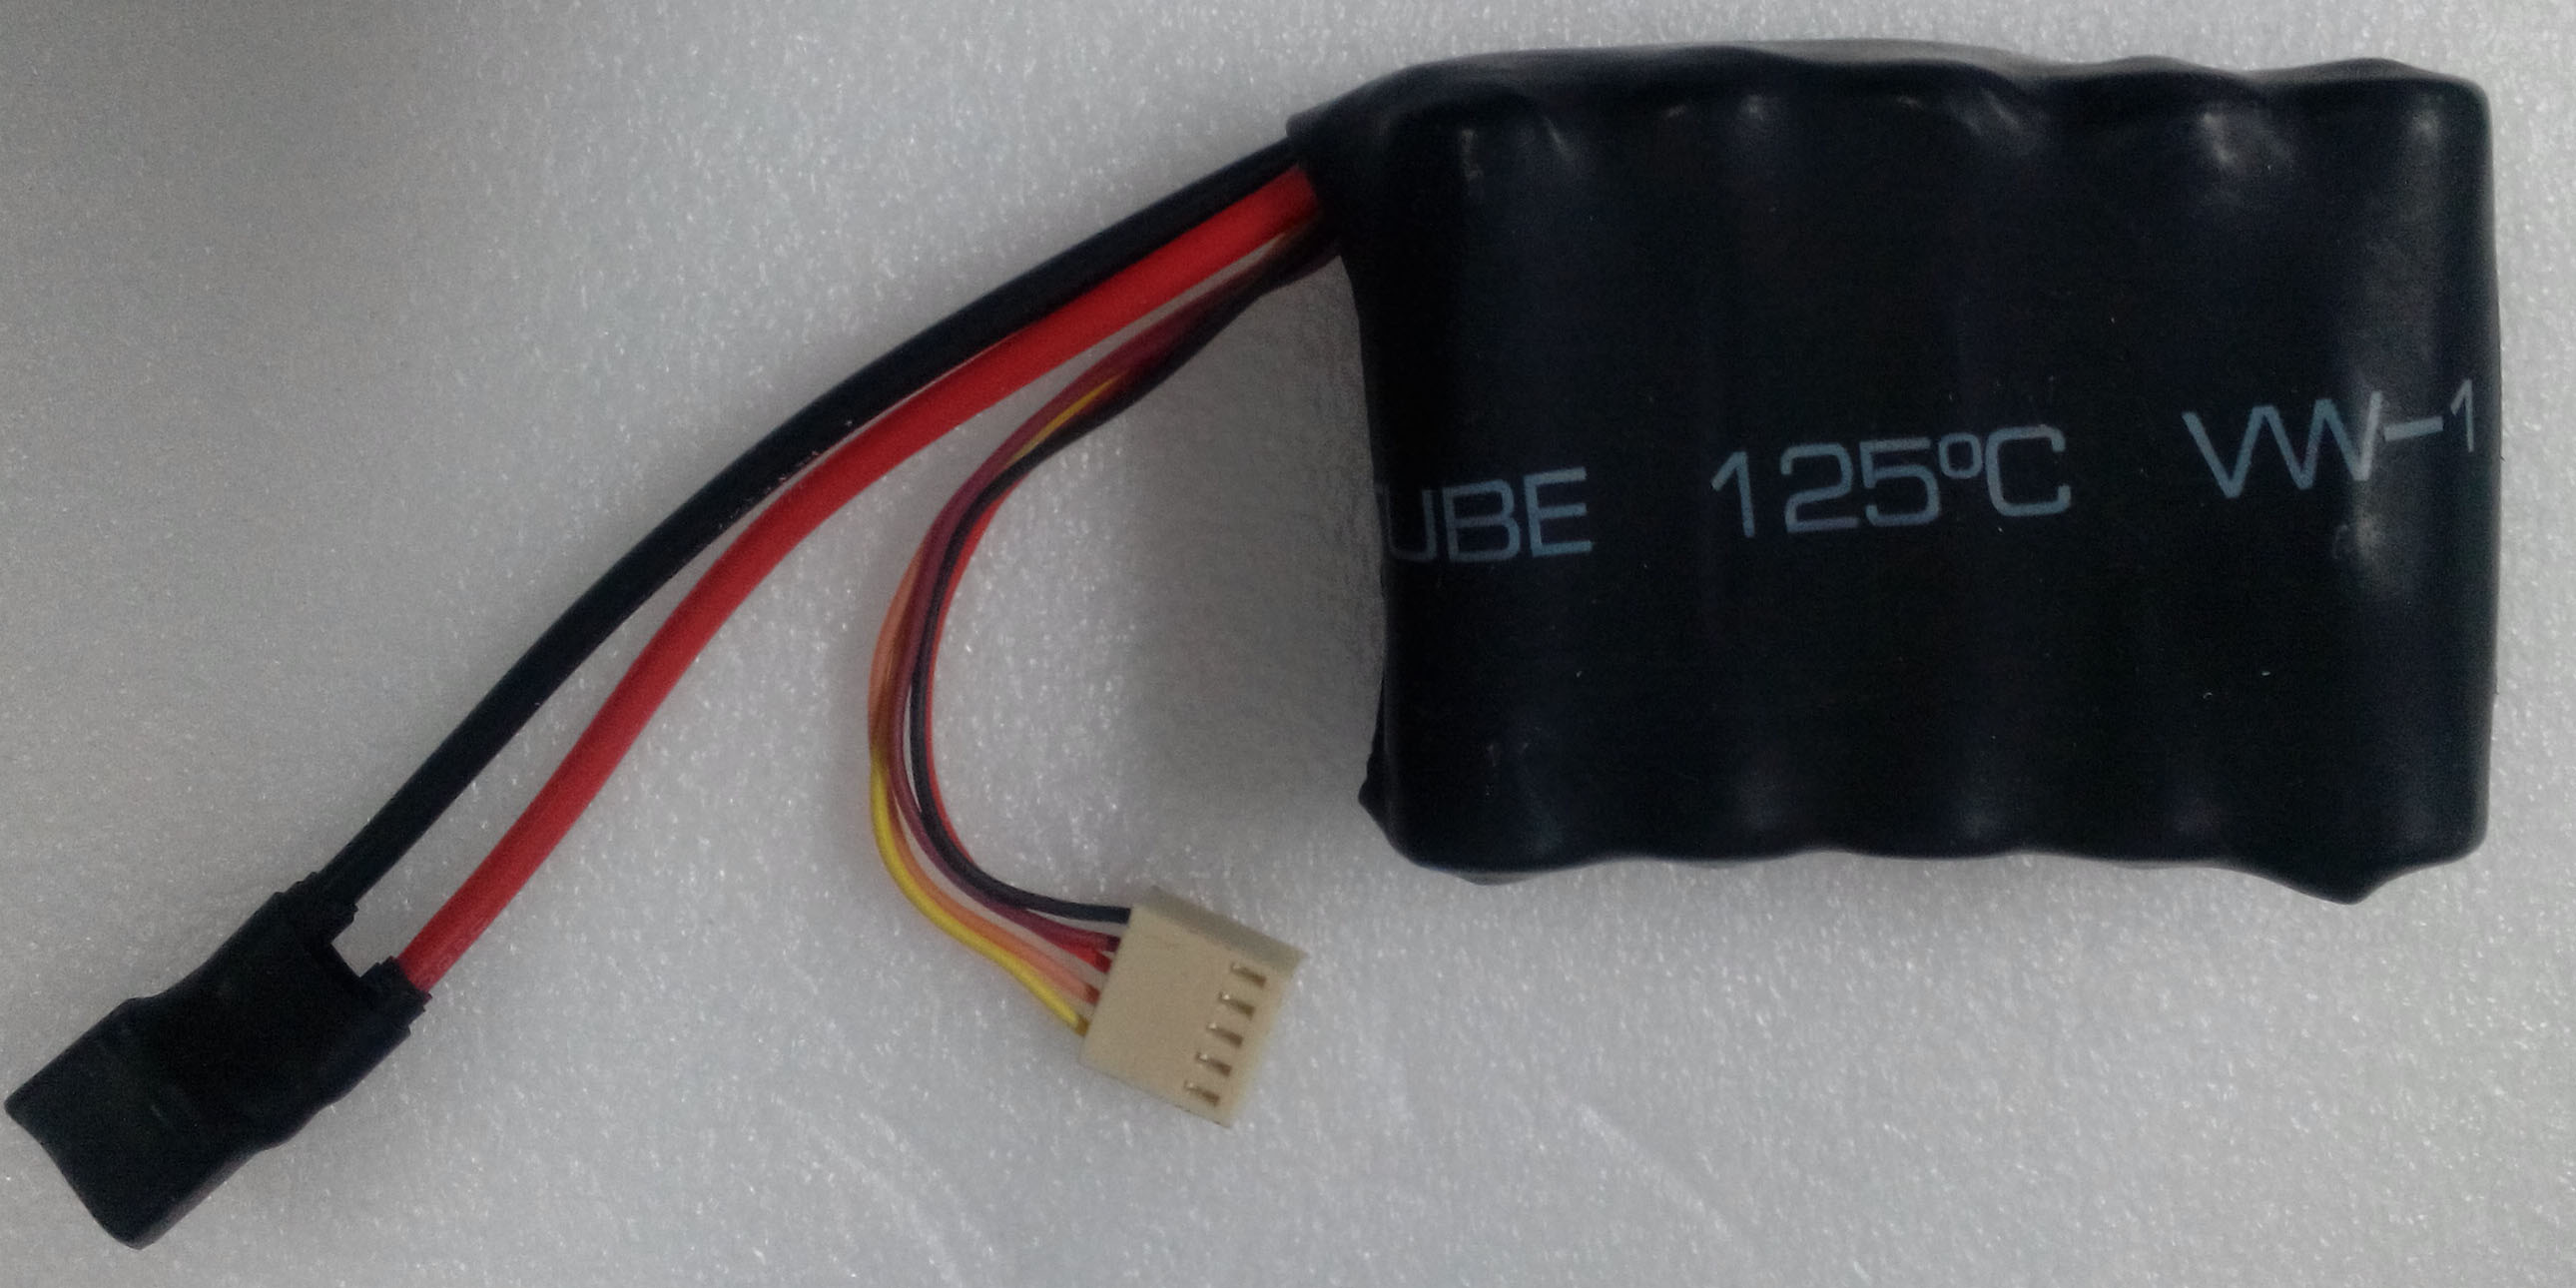
\includegraphics[width=3cm,height=3cm]{battery}
	\end{columns}
	
\end{frame}




% Placing a * after \section means it will not show in the
% outline or table of contents.
\section{Future Work}

\begin{frame}{Future Work}
  \begin{itemize}
  
  \item Interfacing IMU. 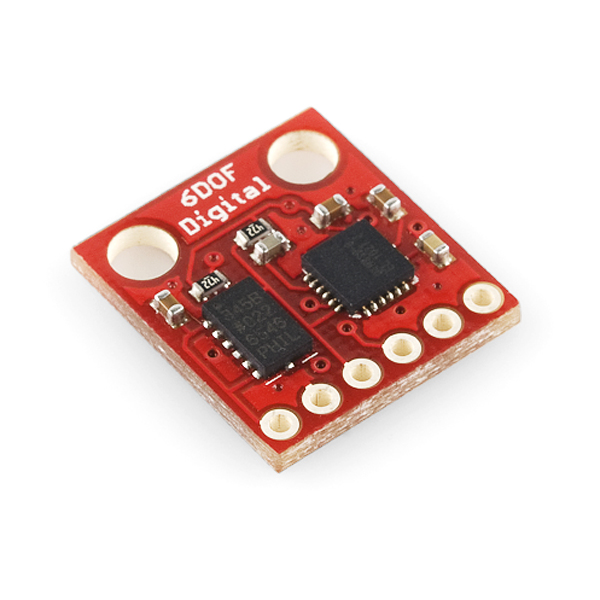
\includegraphics[width=1cm,height=1cm]{imu}
  \item Building a GUI for controlling the robot autonomously.
  \item Interfacing camera along with a smart processor like raspberry pi or a beagle board.
  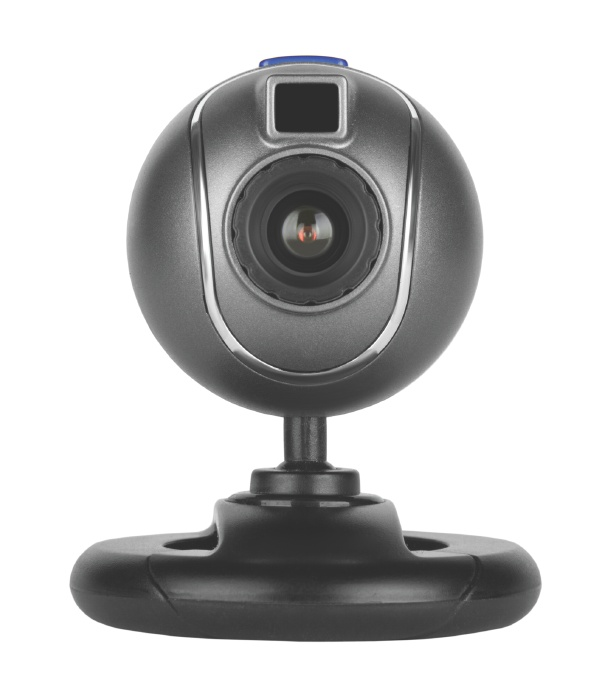
\includegraphics[width=1cm,height=1cm]{Camera}
  
\includegraphics[width=1cm,height=1cm]{Raspi}
  \item Interfacing various sensors like ultrasonic sensors for distance calculation,
  Xbee for wireless communication.
  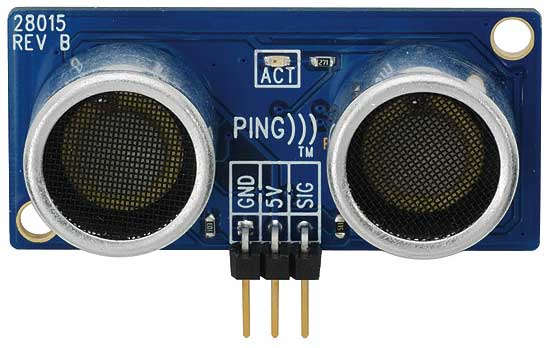
\includegraphics[width=1cm,height=1cm]{ultrasonic}
  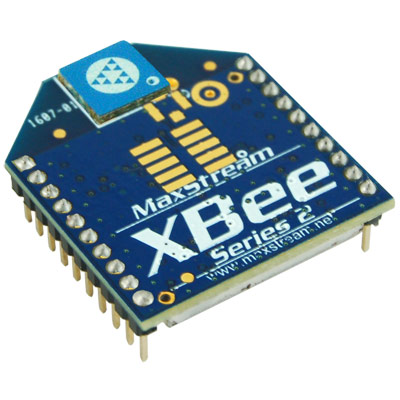
\includegraphics[width=1cm,height=1cm]{XBee-Pro}
  \item Interfacing with modules like Kinect to depict the human motion and many more.
  \end{itemize}
  
  
\end{frame}



% All of the following is optional and typically not needed. 
\section{B.E project idea!}
\begin{frame}{B.E project idea!}
	\begin{itemize}
	\item A four legged Robot.
	\item Micro-quadcopter for surveillance
	\item Interfacing IMU.
	\item Interfacing camera along with a smart processor like raspberry pi with existing Humanoid. 
	\end{itemize}
	
	
\end{frame}



\begin{frame}{End}
	\centering
	
	\Huge{Thank you}
\end{frame}
\end{document}


